\documentclass[12pt]{article}

% for special characters
\usepackage[utf8]{inputenc}
% for images
\usepackage{graphicx}
\graphicspath{{img/}}
% for source in images
\usepackage{floatrow}
% for urls
\usepackage{url}
% for references
\usepackage[sorting=none]{biblatex}
\addbibresource{references.bib}
% for multiple images
\usepackage{subfig}
% for automatic reference prefix
\usepackage{hyperref}
% for uppercase reference at the beginning of a sentence
\usepackage{cleveref}
% for good looking tables
\usepackage{booktabs}

\begin{document}

\title{
\vspace{-2.0cm}

\includegraphics{zhaw}\\ 
\vspace{3cm}
Automated scoring of bone erosion for rheumatoid arthritis with deep neural networks\\
{\Large Zurich University of Applied Sciences}}
\author{\begin{tabular}{rl}
  \textbf{Author:} & Janick Rohrbach \\
  \textbf{Supervisor:} & Dr. Oliver Dürr \\ & Prof. Dr. Beate Sick \\
  \textbf{Industrial Partner:} & Seantis GmbH \\
  \textbf{External Supervisor:} & Fabian Reinhard \\ & Dr. Tobias Reinhard \\
  \textbf{Date:} & December 22, 2017 \\
  \hspace{6.0cm} & \hspace{6.0cm}
\end{tabular}}
\date{}
\maketitle

\newpage

\section*{Declaration of originality\\ \large{Project Thesis at the School of Engineering}}
By submitting this project thesis, the undersigned student confirms that this thesis is his own work and was written without the help of a third party. \\
\\
The student declares that all sources in the text (including Internet pages) and appendices have been correctly disclosed. This means that there has been no plagiarism, i.e. no sections of the project thesis have been partially or wholly taken from other texts and represented as the student’s own work or included without being correctly referenced. \\
\\
Any misconduct will be dealt with according to paragraphs 39 and 40 of the General Academic Regulations for Bachelor’s and Master’s Degree courses at the Zurich University of Applied Sciences (Rahmenprüfungsordnung ZHAW (RPO)) and subject to the provisions for disciplinary action stipulated in the University regulations.\\
\vspace{3cm} \\
Zurich, December 22, 2017 \hspace{5cm} Janick Rohrbach

\newpage

\section*{Abstract}
Abstract goes here

\newpage

\section*{Acknowledgements}
I would like to express my sincere thanks to my supervisors Beate Sick and Oliver Dürr who provided me with guidance and support during the writing of this thesis. 

I would also like to thank Fabian Reinhard and Tobias Reinhard (Seantis GmbH) for their valuable inputs. 

Further, I want to acknowledge the SCQM foundation which made this thesis possible by providing the comprehensive dataset. A list of rheumatology offices and hospitals that are contributing to the SCQM registries can be found on www.scqm.ch/institutions. The SCQM is financially supported by pharmaceutical industries and donors. A list of financial supporters can be found on www.scqm.ch/sponsors.

\newpage

\tableofcontents

\newpage

\section{Introduction}

This thesis shows a method for the automated scoring of x-ray images of patients with rheumatoid arthritis. 

\subsection{Background}

Rheumatoid arthritis is an autoimmune disease. Which means that the disease is caused by a malfunctioning immune system. The immune system attacks healthy tissue instead of bacteria and viruses. This causes inflammation in the joints. Irreversible damage to the bone in the joint can occur, if the inflammation lasts for a long time. \cite{rheuma} Rheumatoid arthritis is incurable, merely the symptoms can be treated.

Today, the severity of the bone erosion is assessed by a trained rheumatologist by using x-ray images of hand and feet. This process takes several minutes per patient. This thesis shows, how recent advances in computer vision make it possible to automate this task. This leads to time savings which in return help the rheumatologist to spend more time with the patient.

The Swiss Clinical Quality Management in Rheumatic Diseases (SCQM) Foundation runs a national registry of inflammatory rheumatic diseases. \cite{scqm_about} They have collected anonymized patient data for over 10 years and provide the x-ray images used for this analysis.

Seantis GmbH, the industrial partner for this thesis, is a Swiss company that develops data driven web applications for medical research, pubic administration and aviation. \cite{seantis_about} For their customer SCQM they want to automate the bone erosion assessment. They already have a working algorithm, which detects the body part shown in the x-ray image. A second algorithm detects the joints in the image and extracts them as single images. These images are then used together with the bone erosion scores to train our model.

% Stand der Technik: Bisherige Lösungen des Problems und deren Grenzen 
% (Nennt kurz den Industriepartner und/oder weitere Kooperationspartner und dessen/deren Interesse am Thema Fragestellung) 

\subsection{Related literature}

% Nennt bestehende Arbeiten/Literatur zum Thema Literaturrecherche

There are several applications where convolutional neural networks are used in medical research.

A recent paper from Tajbakhsh et al. \cite{tajbakhsh_2017} investigated whether fine-tuning a pre-trained CNN is better than training a CNN from scratch when applied to medical images. They find that pre-trained networks with fine-tuning always outperformed or at least performed as well as CNNs trained from scratch. They further recommend a layer-wise fine tuning which seems to outperform shallow and deep tuning.

A study by Paul et al. \cite{paul_2017} tried to classify osteoporosis by considering x-ray images of the bone. This task proved to be very difficult as the x-ray images from healthy patients look very similar to the ones of patients with the disease. By using a transfer learning approach they achieved a validation accuracy of 44.82 \%.

Zhou et al. \cite{zhou_2002} used a two-level ensemble of neural networks to identify lung cancer cells on x-ray images of the chest. The first-level ensemble classifies whether a cell is a cancer cell or not by using full voting. The second-level ensemble is used only on cells classified by the first-level as cancer cells. It differentiates between different cancer classes as well as a non-cancer class. This ensemble works with plurality voting. The authors state that this method achieves a high accuracy and a low rate of false negatives.

A report from Chen \cite{chen_2016} showed the application of convolutional neural networks on x-ray images of hands to predict the developmental bone age. He achieves a top one and two accuracy of 46 \% and 70 \% respectively. This result is close to previously used methods which use manual segmentation and handcrafted features.

In a degree project Hensman and Masko \cite{hensman_2015} looked at the impact of imbalanced training data for CNNs. They find, that heavy imbalances have a strong impact on the performance and suggest oversampling of minority classes to improve the performance of the network.

\subsection{Aim and scope of this thesis}

The aim of this thesis is to predict bone erosion scores from x-ray images. We further examine how the bone erosion and the disease activity are correlated and use a time series of images to predict the course of the disease.

The work is based on images of the left hand only. There also exist images of right hands as well as images of left and right feet. But at this point in time, only the joints of left hands have been extracted from the images. It is assumed that the model will perform similar on the joints of the right hand. By fine-tuning the model on the images of joints from feet it should also perform well for those images.

\subsection{Outline}

\Cref{sec:theory} describes how the joints in the hand are scored and introduces artificial neural networks (ANNs) and the subcategory convolutional neural networks (CNNs). In \autoref{sec:methods} the steps from data preparation to predicting the scores are shown. \autoref{sec:results} presents the results of the predictions which are then discussed in \autoref{sec:discussion}. Finally \autoref{sec:conclusion} concludes this thesis

% (Übersicht über die Arbeit: stellt die folgenden Teile der Arbeit kurz vor)


\newpage

\section{Theory}
\label{sec:theory}

\subsection{Finger joints}
\label{subsec:joints}

\autoref{fig:joints} shows an x-ray image of two hands similar to the images received from the SCQM foundation. The five proximal interphalangeal (PIP) joints and the 5 carpometacarpal (MCP) joints per hand are shown with blue bounding boxes. These are the joints, that are assessed with a score. Usually, the wrist joint is also scored but we limited our analysis to the five PIP joints and the 5 MCP joints.

\begin{figure}[ht]
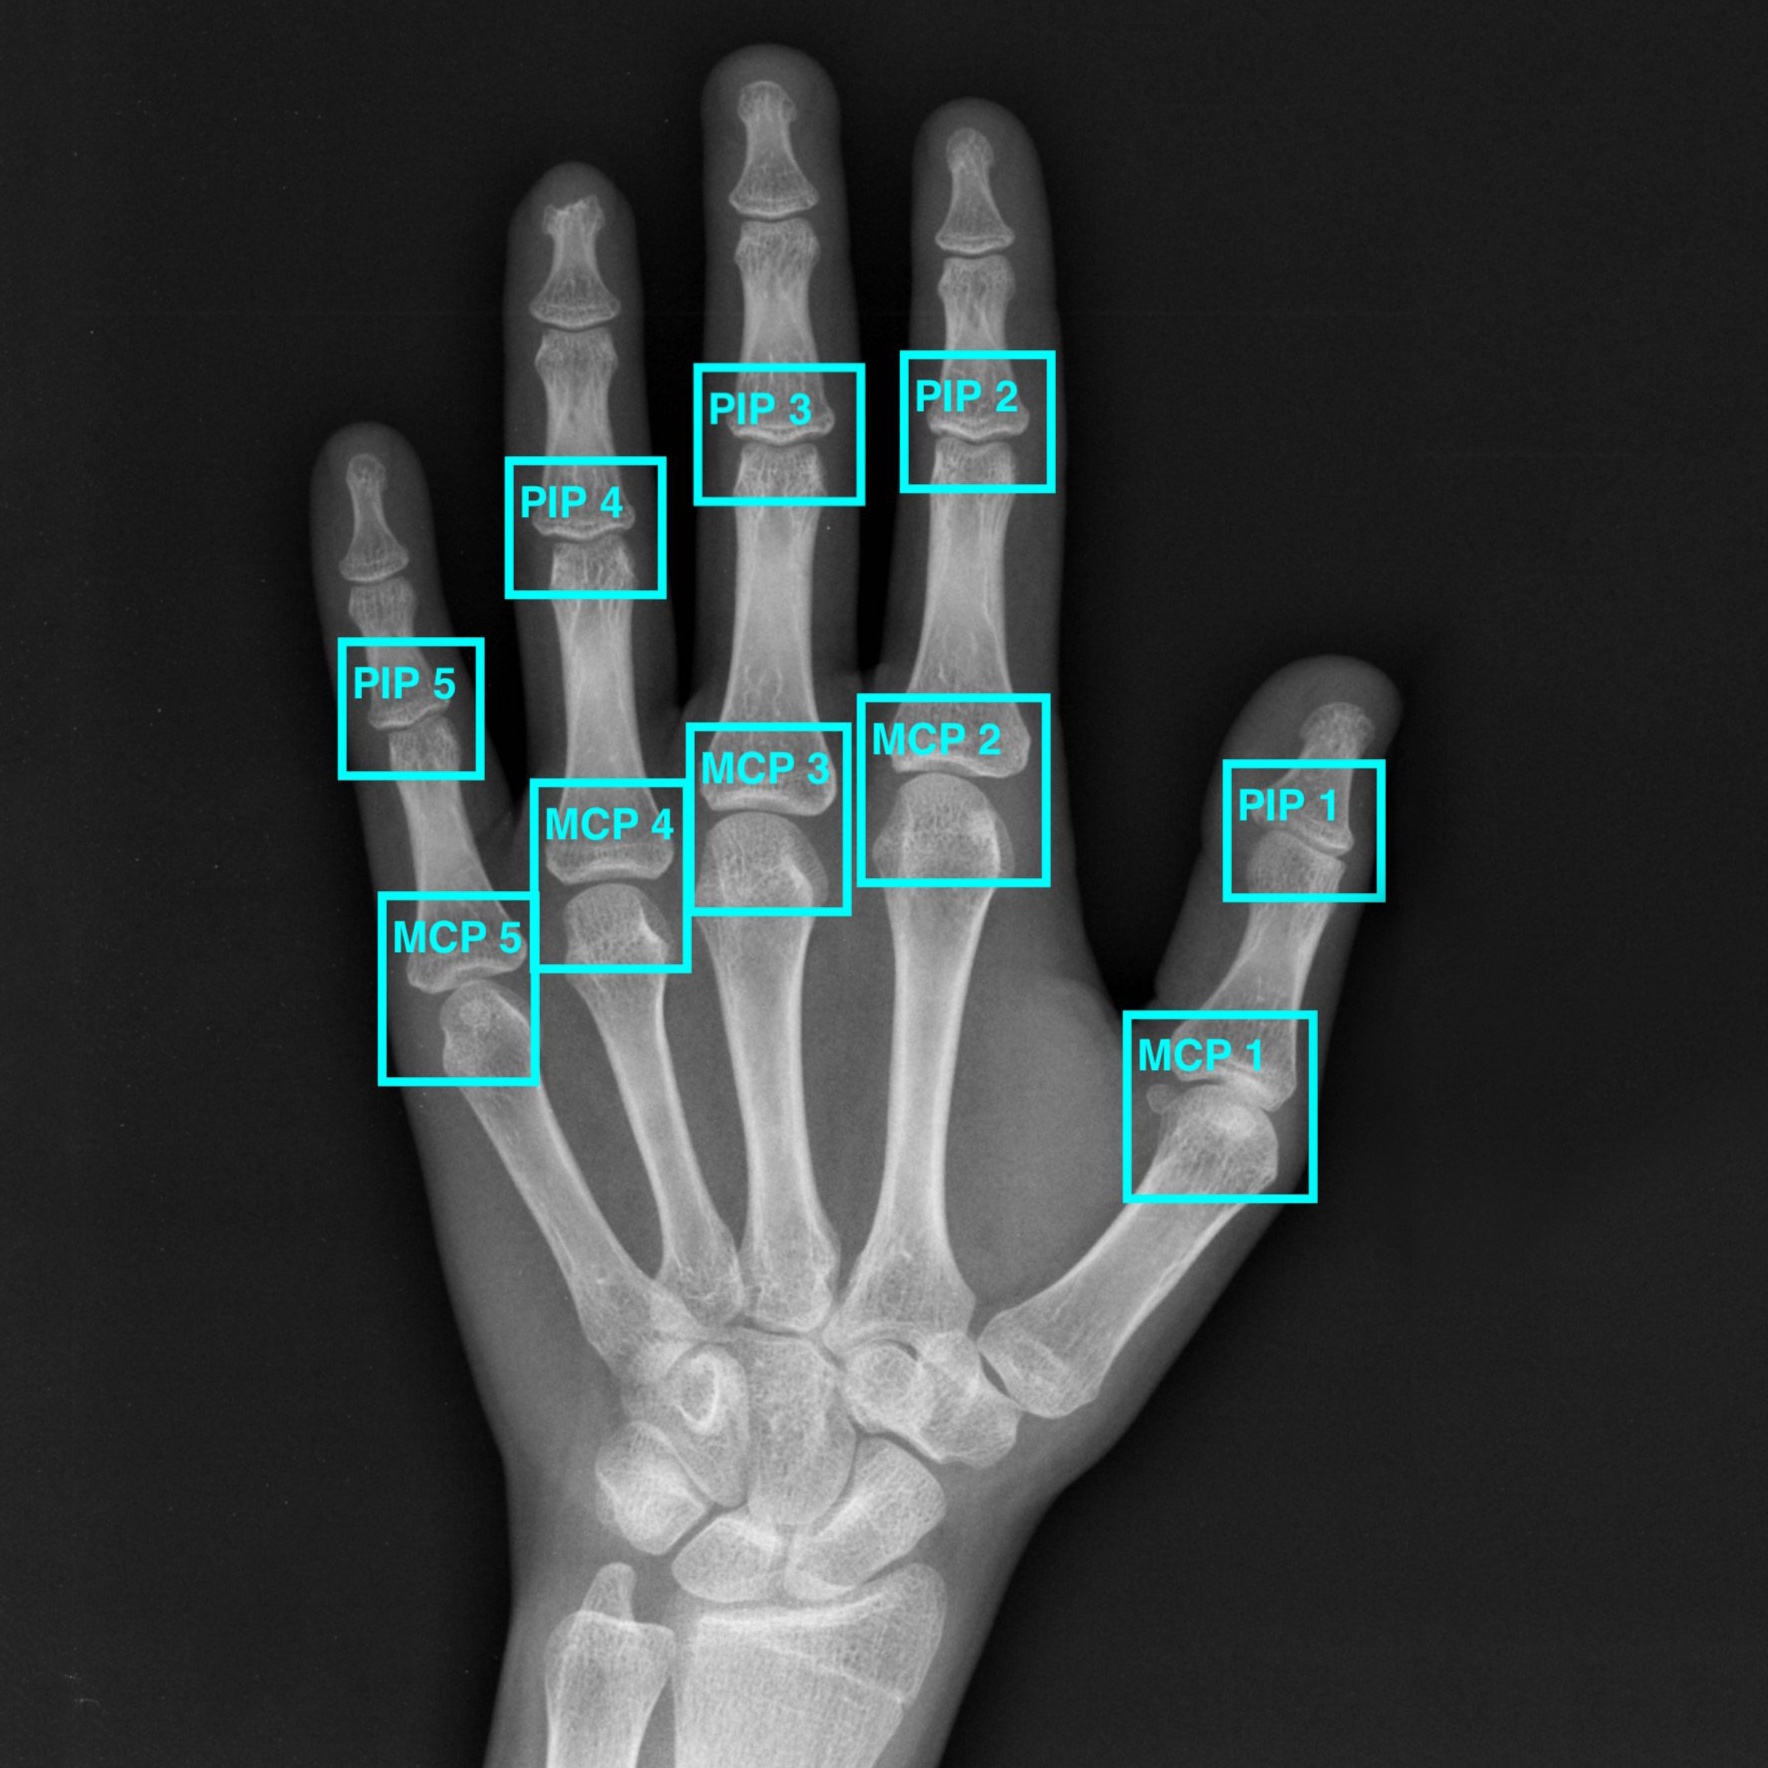
\includegraphics[width=10cm]{joints}	
\caption{Proximal interphalangeal (PIP) joints and carpometacarpal  (MCP) joints.}
\floatfoot{Original image by Nevit Dilmen (CC BY-SA) \url{https://commons.wikimedia.org/wiki/File:Medical\_X\-Ray\_imaging\_OPC06\_nevit.jpg}}
\label{fig:joints}
\end{figure}

\subsection{Ratingen-score}
\label{subsec:ratingen}

The most important criteria for the effectiveness of a treatment is the influence on the radiological progression. To quantify the irreversible bone erosion in the joint, several scoring methods were developed. The score used in this thesis is called Ratingen-score, it estimates the percentage of eroded joint surface. \cite{rau_2007}. The labels of our data lie within 0 and 100 and correspond to the percentage of joint surface erosion. These values can easily be converted to Ratingen-Scores according to \autoref{tab:ratingen}.

\begin{table}[ht]
\centering
\caption{Disease stages of Ratingen-score \cite{rau_2007} }
\label{tab:ratingen}
\begin{tabular}{@{}ll@{}}
\toprule
Stage & Description                                                          \\ \midrule
0     & Normal joint                                                         \\
1     & One or more erosions, less than 20 \% of the joint surface is eroded \\
2     & 21 \% - 40 \% of the joint surface is eroded                         \\
3     & 41 \% - 60 \% of the joint surface is eroded                         \\
4     & 61 \% - 80 \% of the joint surface is eroded                         \\
5     & More than 80 \% of the joint surface is eroded                       \\ \bottomrule
\end{tabular}
\end{table}


\subsection{Artificial neural networks}
\label{subsec:ann}
This section offers a very brief introduction to artificial neural networks. A more in-depth explanation can be found in Andrey Karpathy's course notes for the Stanford class CS231n. \cite{karpathy}

The structure of an Artificial neural network (ANN) is inspired by the human brain. It consists of approximately 100 billion neurons which form an interconnected network. The neurons can communicate with each other by transmitting electrical potential. If the potential in a neuron reaches a certain threshold, it fires and transmits the potential to connected neurons. \cite{kruse_2016}

An ANN is a very simplified model of this biological process. A single neuron can be described by following equation. $$f\left(\sum_{i}w_i*x_i+b\right)$$ Where $x_i$ are the inputs, $w_i$ are the weights and $b$ is a bias term. The activation function $f$ models the firing of the neuron. The activation function used in this thesis is the rectified linear unit (ReLU) which is calculated as follows: $f(x)=max(0,x)$

These single neurons can then be combined to networks. The most simple network is the feed forward neural network described in the following section.

\subsubsection{Feed forward neural networks}
\label{subsubsec:ffnn}
A feed forward neural network (FFNN) has an input layer, arbitrarily many hidden layers and one output layer. The neurons of each layer are connected to every neuron of the next layer. It is called feed forward because data  can only flow in one direction and there are no feedback loops. \autoref{fig:ffnn} shows a possible structure for an FFNN.

\begin{figure}[ht]
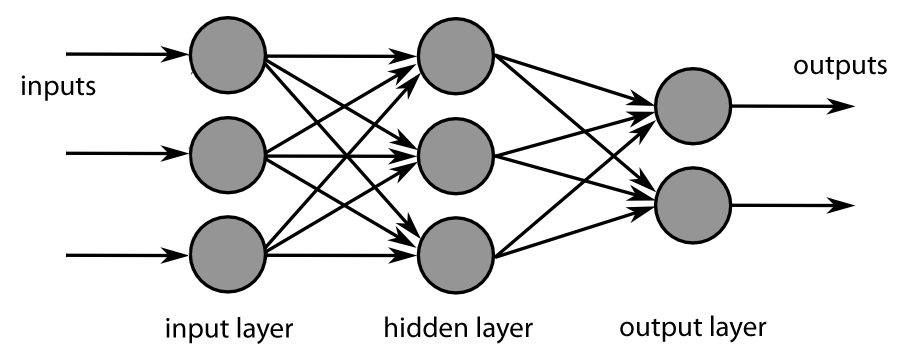
\includegraphics[width=10cm]{ffnn}	
\caption{Feed forward neural network with one hidden layer.}
\floatfoot{Image by Chrislb (CC BY-SA) \url{https://commons.wikimedia.org/wiki/File:MultiLayerNeuralNetworkBigger_english.png}}
\label{fig:ffnn}
\end{figure}

For supervised learning the weights and biases of this network can be trained by using back-propagation. The input is fed through the network with randomly initialized parameters. The output is then compared to the true values by using a loss-function. The loss is then back-propagated through the network to adjust the parameters.

A special type of the FFNN, used for image recognition, is the convolutional neural network, which is described in the next section.

\subsubsection{Convolutional neural networks}
\label{subsubsec:cnn}
Convolutional neural networks (CNNs) take an image as an input. The image can be seen as a 3-dimensional matrix, where the third dimension includes the different color channels. Instead of fully connected layers, convolutional layers are used. Convolutions work as filters that detect different features in the image. These filters usually have a small size (e.g. 3x3) and are moved over the image. The parameters for this filter are always the same, it does not matter where in the image the filter is applied. \autoref{fig:cnn} shows a possible architecture of a CNN with multiple convolutional layers and a fully connected layer at the end.

\begin{figure}[ht]
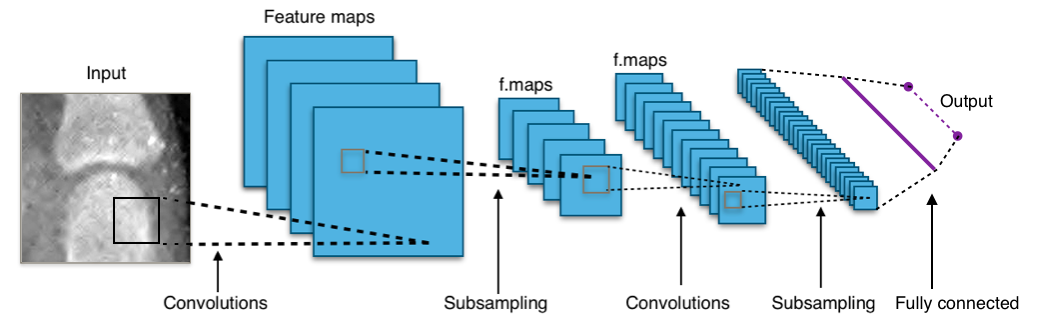
\includegraphics[width=10cm]{cnn}	
\caption{Structure of a convolutional neural network.}
\floatfoot{Original  image by Aphex34 (CC BY-SA) \url{https://commons.wikimedia.org/wiki/File:Typical_cnn.png}}
\label{fig:cnn}
\end{figure}


\newpage
\section{Methods}
\label{sec:methods}

Keras % reference

\subsection{Data preparation}

The pre-processing step formats the images into a suitable format that can be used as an input for the CNN. 

The images of the joints have varying exposure. Some images are very dark while others are very bright. It was therefore considered to apply a histogram equalization, which is a linear transformation that maps the lightest pixel to 255 and the darkest pixel to 1. However, this transformation did not improve the accuracy of the model and was not used for the final model.

The data was randomly split into a training set (70 \% of the data), a test set (20 \% of the data) and a validation set (70 \% of the data). It was split such that all images of the same person are in the same set.

The Rau scores of the labeled joints are highly imbalanced. As seen in \autoref{fig:imbalance} most of the joints are healthy and received a score of 0. There are quite a few observations with scores between 0 and 25 but there are very little observations with scores higher than 25. Because the CNN minimizes the overall loss-function, it would perform bad for the underrepresented part of the data. In this case, the model would be bad in predicting high scores. In order to make the model a good predictor for all cases, we introduced ...????????????

\begin{figure}[ht]
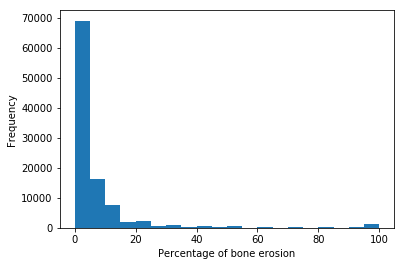
\includegraphics[width=10cm]{imbalance}	
\caption{Distribution of the Rau scores}
\label{fig:imbalance}
\end{figure}

\subsection{Modeling}

Convolution\\
BatchNorm\\
Relu\\
Convolution\\
BatchNorm\\
Relu\\
MaxPooling\\

6x

2 Dense layers

Output layer Softmax

\subsection{Classification}

\begin{figure}[ht]
\begin{tabular}{ccc}
\subfloat[Original data]{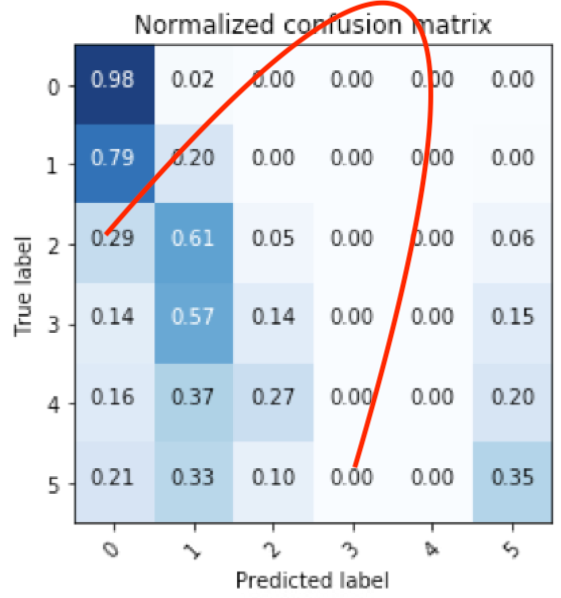
\includegraphics[width = 1.5in]{classification_original}} &
\subfloat[Oversampled]{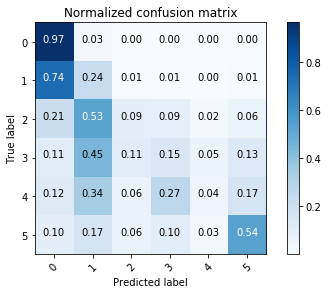
\includegraphics[width = 1.5in]{classification_oversampled}} &
\subfloat[Weights]{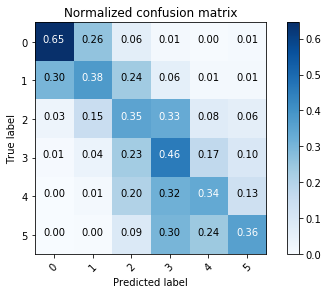
\includegraphics[width = 1.5in]{classification_weights}}
\end{tabular}
\caption{Confusion matrixes for the predictions of the classifcation models.}
\end{figure}

\subsection{Regression}

\begin{figure}[ht]
\begin{tabular}{ccc}
\subfloat[Original data]{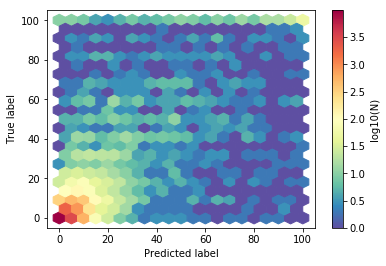
\includegraphics[width = 1.5in]{regression_original}} &
\subfloat[Oversampled]{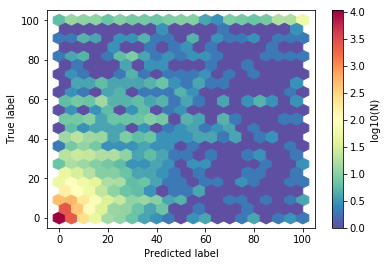
\includegraphics[width = 1.5in]{regression_oversampled}} &
\subfloat[Weights]{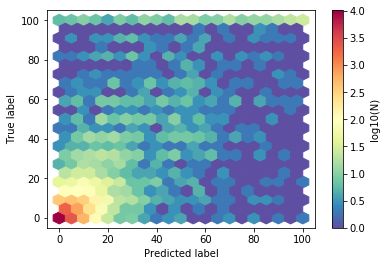
\includegraphics[width = 1.5in]{regression_weights}}
\end{tabular}
\caption{Predictions of the regression models.}
\end{figure}

\newpage
\section{Results}
\label{sec:results}


\newpage
\section{Discussion}
\label{sec:discussion}


\newpage
\section{Conclusion}
\label{sec:conclusion}



\newpage
\printbibliography

\newpage
\listoffigures


\end{document}
